% fig-four-examples.tex
% "Four Faces of Process: Events Mistaken for Things"
% Standalone TikZ figure — Ch. IV
\documentclass[tikz,border=6mm]{standalone}
\usepackage{tikz}
\usepackage{xcolor}
\usetikzlibrary{arrows.meta,calc,decorations.pathmorphing,decorations.markings,shapes.geometric,positioning,backgrounds,fit,shadings,patterns}
\definecolor{substblue}{RGB}{70,130,180}
\definecolor{procamber}{RGB}{180,110,30}
\definecolor{feltgreen}{RGB}{0,110,55}
\definecolor{bgcream}{RGB}{252,248,240}
\definecolor{atomblue}{RGB}{100,160,210}
\definecolor{emphred}{RGB}{160,40,40}
\definecolor{panelborder}{RGB}{180,170,155}

\begin{document}
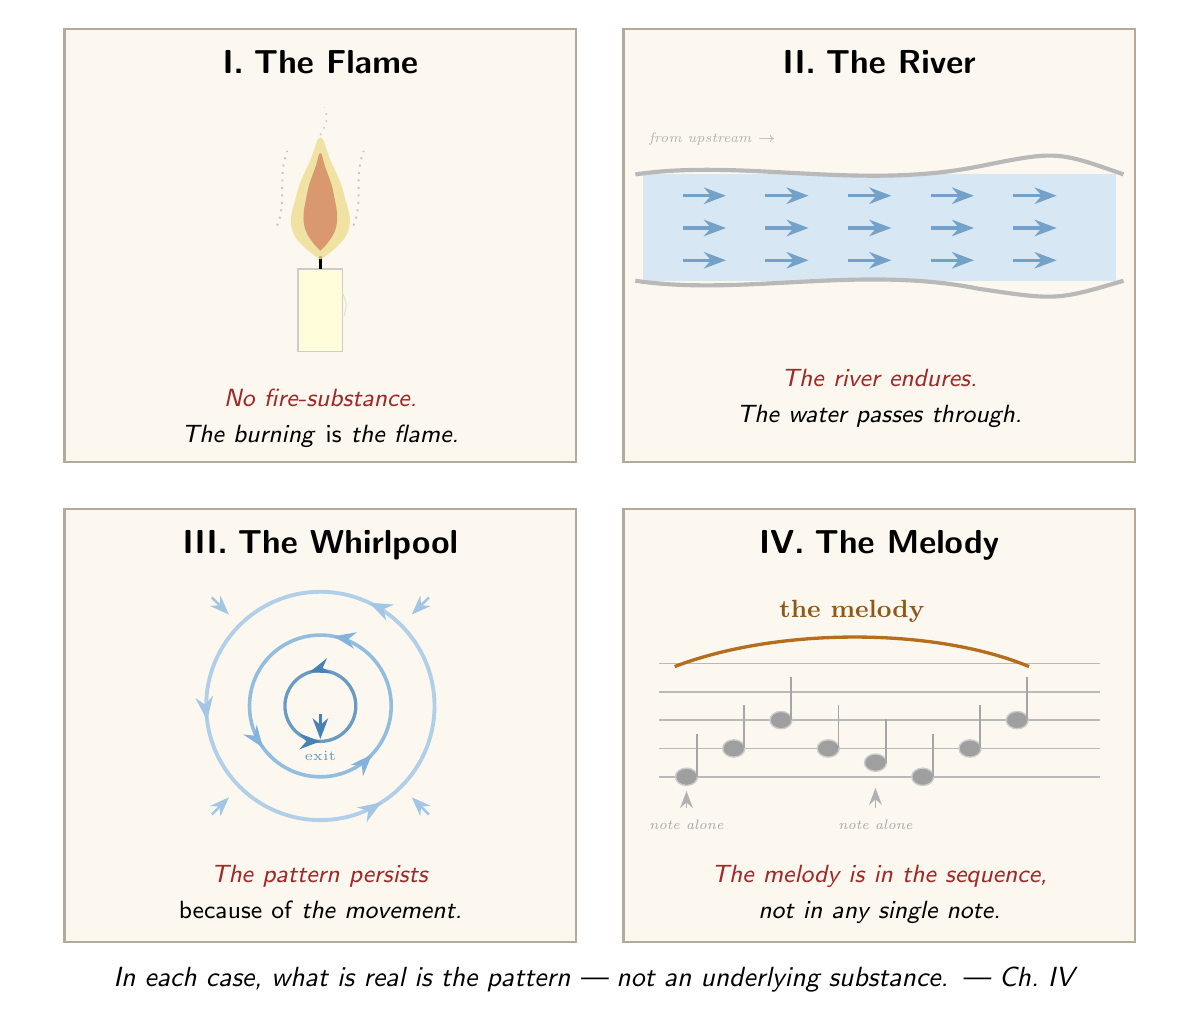
\begin{tikzpicture}[font=\sffamily]

% ── Grid layout constants ────────────────────────────────────────────────────
% Each panel: 6.5 wide × 5.5 tall; gutter: 0.6
% Row 0 (bottom panels): y=0; Row 1 (top panels): y=6.1
% Col 0 (left): x=0; Col 1 (right): x=7.1

% ════════════════════════════════════════════════════════════════════════════
% PANEL 1 (top-left): "The Flame"
% ════════════════════════════════════════════════════════════════════════════
\begin{scope}[shift={(0,6.1)}]
  \fill[bgcream] (0,0) rectangle (6.5,5.5);
  \draw[panelborder, line width=0.8pt] (0,0) rectangle (6.5,5.5);

  % Title
  \node[anchor=north] at (3.25,5.35) {\large\textbf{I.\;The Flame}};

  % ── Candle ────────────────────────────────────────────────────────────────
  \begin{scope}[shift={(3.25,1.40)}]
    % Candle body
    \draw[fill=yellow!15, draw=gray!40, line width=0.6pt]
      (-0.28,0) rectangle (0.28,1.05);
    % Wax drip — tiny accent
    \draw[yellow!20!gray!30, line width=0.4pt]
      (0.28,0.75) .. controls (0.34,0.60) .. (0.30,0.45);
    % Wick
    \draw[black, line width=0.9pt] (0,1.05) -- (0,1.22);

    % ── Outer flame ─────────────────────────────────────────────────────────
    \draw[fill=procamber!50!yellow!45, draw=none, fill opacity=0.82]
      plot[smooth, tension=0.75] coordinates {
        (0,1.17) (0.35,1.52) (0.30,2.00) (0.12,2.45)
        (0,2.72) (-0.12,2.45) (-0.30,2.00) (-0.35,1.52) (0,1.17)
      };

    % ── Inner flame ─────────────────────────────────────────────────────────
    \draw[fill=procamber!80!red!65, draw=none, fill opacity=0.92]
      plot[smooth, tension=0.75] coordinates {
        (0,1.28) (0.20,1.58) (0.17,2.00) (0.06,2.35)
        (0,2.52) (-0.06,2.35) (-0.17,2.00) (-0.20,1.58) (0,1.28)
      };

    % ── Heat shimmer lines ───────────────────────────────────────────────────
    \foreach \xsh/\xend in {-0.55/-0.42, 0.42/0.55}{
      \draw[gray!45, dotted, line width=0.7pt]
        (\xsh,1.60) .. controls (\xend,1.90) and (\xsh,2.20) .. (\xend,2.55);
    }
    \draw[gray!40, dotted, line width=0.6pt]
      (0,2.75) .. controls (0.10,2.95) .. (0.05,3.10);
  \end{scope}

  % Caption
  \node[anchor=north, text width=5.6cm, align=center] at (3.25,1.05)
    {\small\textcolor{emphred}{\textit{No fire-substance.}}\\[1pt]
     \small\textit{The burning \emph{is} the flame.}};
\end{scope}

% ════════════════════════════════════════════════════════════════════════════
% PANEL 2 (top-right): "The River"
% ════════════════════════════════════════════════════════════════════════════
\begin{scope}[shift={(7.1,6.1)}]
  \fill[bgcream] (0,0) rectangle (6.5,5.5);
  \draw[panelborder, line width=0.8pt] (0,0) rectangle (6.5,5.5);

  % Title
  \node[anchor=north] at (3.25,5.35) {\large\textbf{II.\;The River}};

  % ── River banks and water ────────────────────────────────────────────────
  \begin{scope}[shift={(0,1.60)}]
    % Water fill between y=0.70 and y=2.05
    \fill[atomblue!25]
      (0.25,0.70) -- (6.25,0.70) -- (6.25,2.05) -- (0.25,2.05) -- cycle;

    % Top bank (wavy)
    \draw[gray!55, very thick, line width=1.5pt]
      (0.15,2.05) .. controls (1.5,2.25) and (3.0,1.85) ..
      (4.5,2.15) .. controls (5.5,2.35) .. (6.35,2.05);
    % Bottom bank (wavy)
    \draw[gray!55, very thick, line width=1.5pt]
      (0.15,0.70) .. controls (1.5,0.50) and (3.0,0.90) ..
      (4.5,0.60) .. controls (5.5,0.45) .. (6.35,0.70);

    % Flow arrows
    \foreach \ypos in {0.96, 1.37, 1.78}{
      \foreach \xpos in {0.75, 1.80, 2.85, 3.90, 4.95}{
        \draw[substblue!75, ->, >=Stealth, line width=1.1pt]
          (\xpos,\ypos) -- (\xpos+0.55,\ypos);
      }
    }

    % "from upstream" label — single-line, fits above the river
    \node[font=\tiny\itshape, anchor=west, text=gray!60] at (0.20,2.50)
      {from upstream $\rightarrow$};
  \end{scope}

  % Caption
  \node[anchor=north, text width=5.6cm, align=center] at (3.25,1.30)
    {\small\textcolor{emphred}{\textit{The river endures.}}\\[1pt]
     \small\textit{The water passes through.}};
\end{scope}

% ════════════════════════════════════════════════════════════════════════════
% PANEL 3 (bottom-left): "The Whirlpool"
% ════════════════════════════════════════════════════════════════════════════
\begin{scope}[shift={(0,0)}]
  \fill[bgcream] (0,0) rectangle (6.5,5.5);
  \draw[panelborder, line width=0.8pt] (0,0) rectangle (6.5,5.5);

  % Title
  \node[anchor=north] at (3.25,5.35) {\large\textbf{III.\;The Whirlpool}};

  \begin{scope}[shift={(3.25,3.00)}]
    % Three concentric rings suggesting rotation, colored atomblue→substblue
    % Outer ring
    \draw[atomblue!50, line width=1.4pt,
          postaction={decorate,
            decoration={markings,
              mark=at position 0.18 with {\arrow[atomblue!60,line width=1.2pt]{Stealth}},
              mark=at position 0.52 with {\arrow[atomblue!60,line width=1.2pt]{Stealth}},
              mark=at position 0.84 with {\arrow[atomblue!60,line width=1.2pt]{Stealth}}
            }
          }]
      (0,0) circle (1.45);

    % Middle ring
    \draw[atomblue!70, line width=1.3pt,
          postaction={decorate,
            decoration={markings,
              mark=at position 0.22 with {\arrow[atomblue!80,line width=1.1pt]{Stealth}},
              mark=at position 0.60 with {\arrow[atomblue!80,line width=1.1pt]{Stealth}},
              mark=at position 0.88 with {\arrow[atomblue!80,line width=1.1pt]{Stealth}}
            }
          }]
      (0,0) circle (0.90);

    % Inner ring
    \draw[substblue!80, line width=1.2pt,
          postaction={decorate,
            decoration={markings,
              mark=at position 0.30 with {\arrow[substblue,line width=1.0pt]{Stealth}},
              mark=at position 0.75 with {\arrow[substblue,line width=1.0pt]{Stealth}}
            }
          }]
      (0,0) circle (0.45);

    % Inflow arrows at outer edge (4 directions)
    \foreach \ang in {45,135,225,315}{
      \draw[atomblue!60, ->, >=Stealth, line width=0.9pt,
            shorten >=4pt]
        ({1.95*cos(\ang)},{1.95*sin(\ang)}) --
        ({1.50*cos(\ang)},{1.50*sin(\ang)});
    }

    % Downward exit arrow at center
    \draw[substblue, ->, >=Stealth, line width=1.0pt]
      (0,-0.10) -- (0,-0.42);
    \node[below, font=\tiny, text=substblue!80] at (0,-0.45) {exit};
  \end{scope}

  % Caption
  \node[anchor=north, text width=5.6cm, align=center] at (3.25,1.10)
    {\small\textcolor{emphred}{\textit{The pattern persists}}\\[1pt]
     \small\textit{\emph{because of} the movement.}};
\end{scope}

% ════════════════════════════════════════════════════════════════════════════
% PANEL 4 (bottom-right): "The Melody"
% ════════════════════════════════════════════════════════════════════════════
\begin{scope}[shift={(7.1,0)}]
  \fill[bgcream] (0,0) rectangle (6.5,5.5);
  \draw[panelborder, line width=0.8pt] (0,0) rectangle (6.5,5.5);

  % Title
  \node[anchor=north] at (3.25,5.35) {\large\textbf{IV.\;The Melody}};

  \begin{scope}[shift={(0.45,2.10)}]
    % Staff width
    \def\sw{5.60}

    % ── Five staff lines ────────────────────────────────────────────────────
    \foreach \k in {0,1,2,3,4}{
      \draw[gray!55, line width=0.6pt] (0,{\k*0.36}) -- (\sw,{\k*0.36});
    }

    % ── Note positions: (x, staff-slot) where slot 0=bottom line, 0.5=space
    % C-E-G-E-D-C-E-G  (ascending/descending melody feel)
    % Staff slots: C4=0, D=0.5, E=1, F=1.5, G=2, A=2.5, B=3, C5=4
    % Map slot to y: y = slot * 0.18
    \def\notescale{0.18}
    % (x, slot)
    \foreach \xn/\slot in {
      0.35/0,   % C
      0.95/1,   % E
      1.55/2,   % G
      2.15/1,   % E
      2.75/0.5, % D
      3.35/0,   % C
      3.95/1,   % E
      4.55/2    % G
    }{
      \pgfmathsetmacro{\yn}{\slot*\notescale*2}
      % Note head
      \draw[fill=gray!75, draw=gray!40, line width=0.5pt]
        (\xn,\yn) ellipse (0.14 and 0.11);
      % Stem (upward for slots ≤ 2, else downward)
      \pgfmathparse{\slot <= 2 ? 1 : 0}
      \ifnum\pgfmathresult=1
        \draw[gray!70, line width=0.7pt]
          (\xn+0.13,\yn) -- (\xn+0.13,\yn+0.55);
      \else
        \draw[gray!70, line width=0.7pt]
          (\xn-0.13,\yn) -- (\xn-0.13,\yn-0.55);
      \fi
    }

    % ── Slur over all notes ─────────────────────────────────────────────────
    \draw[procamber, line width=1.2pt]
      (0.20,1.40) .. controls (1.50,1.90) and (3.50,1.90) .. (4.70,1.40);

    % Bracket label
    \node[procamber!80!black, font=\small\bfseries] at (2.45,2.10)
      {the melody};

    % "note alone" arrows for two individual notes
    \draw[gray!60, ->, >=Stealth, line width=0.7pt]
      (0.35,-0.40) -- (0.35,-0.18);
    \node[below, font=\tiny\itshape, text=gray!70] at (0.35,-0.42)
      {note alone};

    \draw[gray!60, ->, >=Stealth, line width=0.7pt]
      (2.75,-0.40) -- (2.75,-0.14);
    \node[below, font=\tiny\itshape, text=gray!70] at (2.75,-0.42)
      {note alone};
  \end{scope}

  % Caption
  \node[anchor=north, text width=5.6cm, align=center] at (3.25,1.10)
    {\small\textcolor{emphred}{\textit{The melody is in the sequence,}}\\[1pt]
     \small\textit{not in any single note.}};
\end{scope}

% ── CAPTION below entire 2×2 grid ───────────────────────────────────────────
\node[anchor=north, text width=14.2cm, align=center] at (6.75,-0.20)
  {\textit{In each case, what is real is the pattern --- not an underlying substance. --- Ch.~IV}};

\end{tikzpicture}
\end{document}
